\Exercise[number={9}]
Consider a one-dimensional binary decision problem, in which the conditional
densities are described by the Cauchy distribution:
\[
    p(x|w_i)=\frac{1}{\pi b}\frac{1}{1+\bigl(\frac{x-a_i}{b}\bigr)^2}
\]
Define a Bayesian classifier and determine the decision criterion,
assuming that \(Pr(w_1)=p\).\\
Draw \(p(w_1|x)\) and \(p(w_2|x)\) for \(a_1=3\), \(a_2=5\), \(b=1\),
\(p=0.5\).

\Answer[number={9}]
The decision criterion \(z(x)\) can be written as:
\begin{align*}
    z(x)
    &=\frac{\log{p(x|w_1)}}{\log{p(x|w_2)}}+\log{\frac{Pr(w_1)}{Pr(w_2)}}
    =\log{p(x|w_1)}-\log{p(x|w_2)}+\log{\frac{p}{1-p}}\\
    &=-\cancel{\log{\pi b}}-\log{\biggl[1+\biggl(\frac{x-a_1}{b}\biggr)^2\biggr]}+\cancel{\log{\pi b}}+\log{\biggl[1+\biggl(\frac{x-a_2}{b}\biggr)^2\biggr]}+\log{\frac{p}{1-p}}
\end{align*}
Then, the decision boundary for the given values is obtained by setting
\(z(x)\) equal to 0:
\begin{align*}
    z(x)=0
    &\Rightarrow
    -\log{\bigl[1+(x-3)^2\bigr]}+\log{\bigl[1+(x-5)^2\bigr]}+\cancel{\log{\frac{0.5}{0.5}}}=0\\
    &\Rightarrow
    \cancel{1}+(x-3)^2=\cancel{1}+(x-5)^2\\
    &\Rightarrow
    \cancel{x^2}+9-6x-\cancel{x^2}-25+10x=0\\
    &\Rightarrow
    4x=16
    \Rightarrow
    x=4
\end{align*}
Such a result is consistent with the general formula for \(Pr(w_1)=Pr(w_2)\),
stating that:
\begin{align*}
    x=\frac{a_1+a_2}{2}=\frac{3+5}{2}=\frac{8}{2}=4
\end{align*}
In order to estimate the posterior probabilities \(p(w_1|x)\) and \(p(w_2|x)\)
let's recall that:
\begin{align*}
    p(w_i|x)=\frac{1}{1+e^{-z_i(x)}}=\sigma_i(x)
    \quad\Longrightarrow\quad
    \text{sigmoid function}
\end{align*}
where
\begin{align*}
    z_1(x)=\log{\frac{1+(x-5)^2}{1+(x-3)^2}}
    \quad\text{and}\quad
    z_2(x)=\log{\frac{1+(x-3)^2}{1+(x-5)^2}}
\end{align*}
Let's study the function \(\sigma_1(x)=p(w_1|x)\):
\begin{itemize}
    \item\quad Domain: \(\mathfrak{D}=\mathbf{R}\)
    \item\quad Sign: \(\sigma_1(x)>0 \quad\forall{x}\in \mathbf{R}\)
    \item\quad Asymptotes:
    \begin{align*}
        \lim_{x\to{+\infty}}{\sigma_1(x)}=\frac{1}{2}
        \quad\text{and}\quad
        \lim_{x\to{-\infty}}{\sigma_1(x)}=\frac{1}{2}
    \end{align*}
    \item\quad Intersection with y-axis:
    \begin{align*}
        \sigma_1(0)
        =\frac{1}{1+e^{-\log{\frac{1+(0-5)^2}{1+(0-3)^2}}}}
        =\frac{1}{1+e^{-\log{\frac{26}{10}}}}
        =\frac{1}{1+\frac{26}{10}}
        =\frac{26}{36}
        \simeq 0.72
    \end{align*}
    \item\quad Decision criterion:
    \begin{align*}
        \sigma_1(x)=0.5
        \Rightarrow
        \frac{1}{1+\frac{x^2-6x+10}{x^2-10x+26}}=\frac{1}{2}
        \Rightarrow
        x=4
    \end{align*}
    \item\quad Maximum and minimum:
    \begin{align*}
        \sigma_1(x)
        =\frac{1}{1+e^{-\log{\frac{1+(x-5)^2}{1+(x-3)^2}}}}
        =\frac{x^2-10x+26}{2x^2-16x+36}
    \end{align*}
    \begin{align*}
        &\Rightarrow
        \frac{d\,\sigma_1(x)}{d\,x}
        =\frac{(2x-10)(2x^2-16x+36)-(x^2-10x+26)(4x-16)}{\cancel{(2x^2-16x+36)^2}}
        >0\\
        &\Rightarrow
        \cancel{4x^3}-20x^2-32x^2+\cancel{160x}+72x-360-\cancel{4x^3}+16x^2+40x^2-\cancel{160x}-104x+416>0\\
        &\Rightarrow
        x^2-8x+14>0\\
        &\Rightarrow
        x_{1,2}=4\pm\sqrt{16-14}=4\pm\sqrt{2}
    \end{align*}
    \(4-\sqrt{2}\quad\Rightarrow\quad\)maximum\(\quad\Rightarrow\quad\sigma_1(4-\sqrt{2})=0.854\)\\
    \(4+\sqrt{2}\quad\Rightarrow\quad\)minimum\(\quad\Rightarrow\quad\sigma_1(4+\sqrt{2})=0.146\)
\end{itemize}
The plot of \(\sigma_1(x)=p(w_1|x)\) is then:
\begin{figure}[H]
    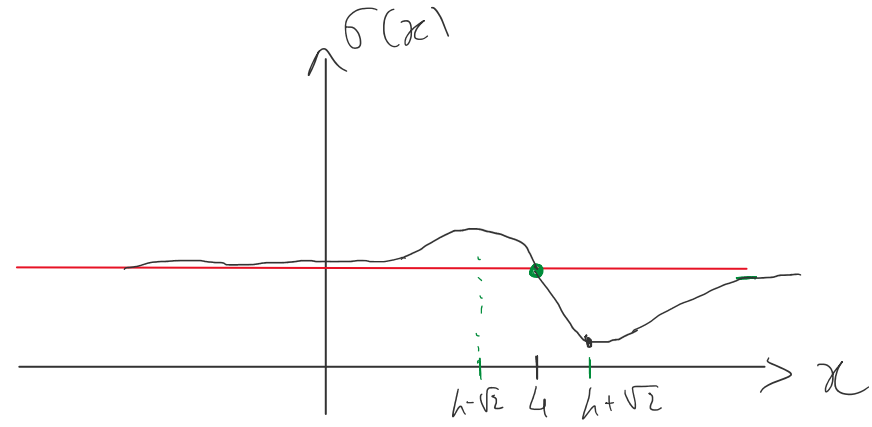
\includegraphics[scale=0.6]{C_9}
    \centering
\end{figure}
Notice that the plot of \(\sigma_2(x)=p(w_2|x)\) is symmetric to
\(\sigma_1(x)\) with respect to a symmetric axis defined as \(x=4\).